\graphicspath{{content/1_literatureReview/figures/}}
\section{Ultrasonic Sensors}

\subsection{Interface}

The HC-SR04 ultrasonic ranging module's interface will be discussed. It has 4 pins, namely \textit{$V_{cc}$, GND, Trig (Trigger)} and \textit{Echo}.
It should be powered with 5 ${V_{dc}}$ and requires at least 15 mA to function, meaning it will dissipate 75 mW of power. 
First, \textit{Trig} should be pulled high to indicate that the device should send a burst of ultrasonic sound out.
Then, if the sound wave is received back, the device will output a distance-proportional pulse on the \textit{Echo} pin.

\begin{figure}[!htb]
  \centering
  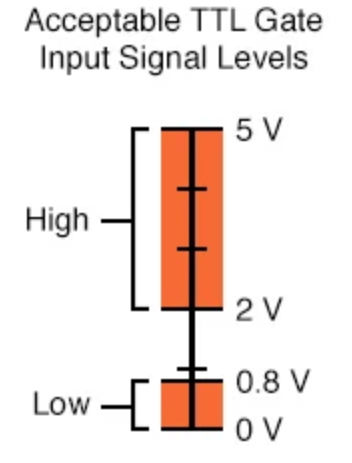
\includegraphics[width=0.15\textwidth]{sonicSensor_TTL}
  \caption{TTL Input/Output Levels \cite{ttlLevels}}
  \label{fig:sonicSensor_TTL}
\end{figure}

The following detailed procedure should be followed to make a distance measurement \cite{datasheetHCSR04}:
\begin{enumerate}
    \item A pulse of at least \SI{10}{\micro\second} should be output onto \textit{Trig}. This pulse must be TTL compliant as indicated
    in Figure \ref{fig:sonicSensor_TTL} i.e. between 2 and 5 V.
    \item If the sound wave is received back by the sensor, \textit{Echo} (also TTL) will go high for ${t_{high}}$ seconds, where ${t_{high}}$ is the time it took the wave to return to the sensor.
          This signal should therefore be conditioned if a circuit which requires 3.3 V is used.
    \item The distance can then be calculated. One of the following methods may be used:
    \begin{enumerate}
        \item The length of time of the \textit{Echo} output signal can be digitally measured and the distance then calculated using \inlineequation[eqn:sensor_distanceFormula]{Distance = \frac{t_{high} * v_{sound}}{2}} \cite{datasheetHCSR04}.
        \item The output pulse can be converted to an analog signal using filtering. The resultant filtered voltage will also be proportional to $t_{high}$.
    \end{enumerate}
    \item A minimum of 60 ms should be present in between each pulse. This allows for a theoretical range of $\frac{\SI{60}{\milli\second} * \SI{340}{m.s^{-1}}}{2} = \SI{10.2}{\metre}$.
          In practice, the device has a range of $\approx 4 m$.
\end{enumerate}

\begin{figure}[!htb]
  \centering
  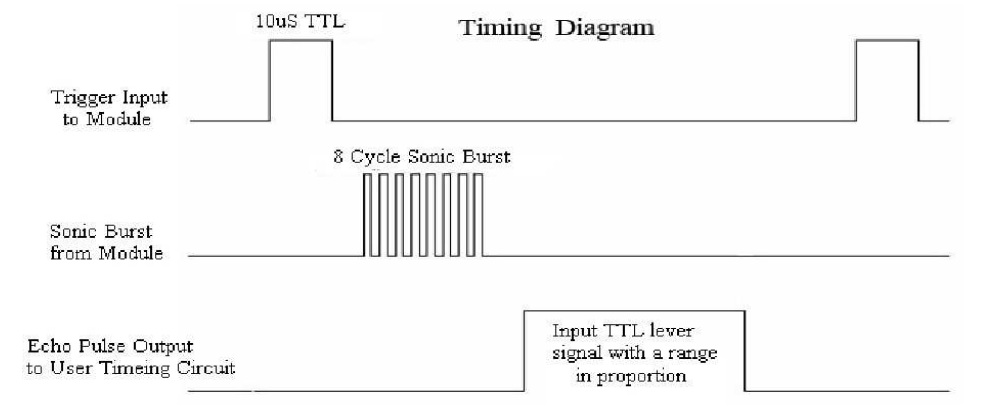
\includegraphics[width=0.4\textwidth]{sonicSensor_timing}
  \caption{Sensor Timing Diagram \cite{datasheetHCSR04}}
  \label{fig:sonicSensor_timing}
\end{figure}

\subsection{Fundamental Operation}

\subsubsection{Sound Transducers}

Ultrasonic sensors work by emitting and receiving sound waves of a high frequency. Electrical "transducers" are used to convert between electrical/sound energy.
These are either excited by an electrical signal and caused to vibrate, or vibrate due to an incoming sound-wave and then generate an electrical signal.
The two main transducer types used in ultrasound include \cite{ultrasonicSensorWorkings}:
\begin{itemize}
    \item \textit{Piezoelectric} transducers. These use a vibrating crystal quartz which deforms in response to a changing potential difference.
    \item \textit{Capacitive} transducers. These make use of a flexible dielectric membrane attached to an electrode. This electrode is attracted and repelled
          by electrical charges.
\end{itemize}

\begin{figure}[!htb]
    \centering
    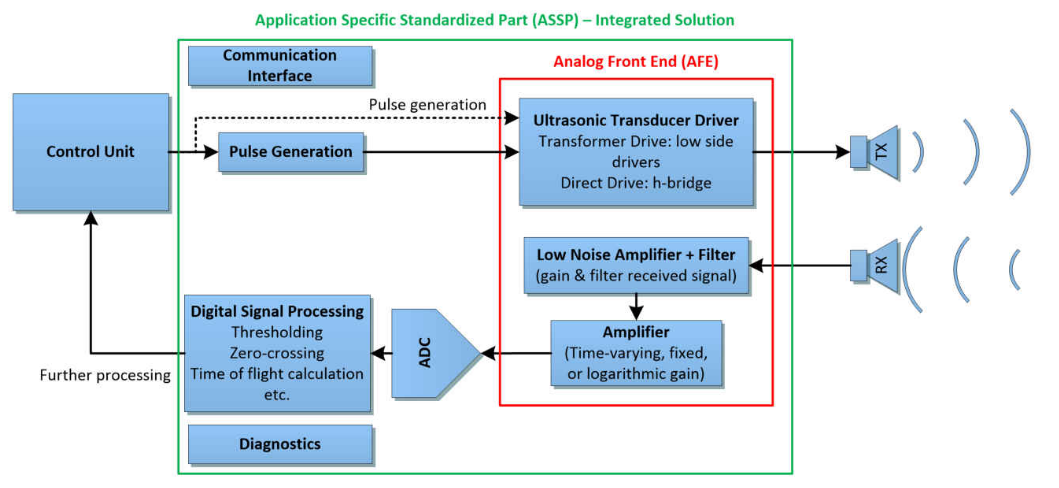
\includegraphics[width=0.55\textwidth]{sonicSensor_system}
    \caption{Simple Ultrasonic Sensing System \cite{ultrasonicSensorBasics}}
    \label{fig:sonicSensor_system}
  \end{figure}

\subsubsection{Pulse Generation}

Ultrasonic systems generally contain a digital control unit \cite{ultrasonicSensorBasics}. This unit is responsible for receiving the trigger signal from the communication interface and generating
a pulse to send to the Analog Front End (AFE). This pulse is usually sinusoidal and is at a much higher frequency than the trigger input (between 30 kHz and 5 MHz).
After the digital pulse is generated, the AFE amplifies it using a transistor drive circuit.
This can be at a relatively low voltage e.g. 5 V, but often high-voltage and "direct drive" amplification is used, which may allow up to 36 V.

\subsubsection{Pulse Acquisition}
After some time, the pulse may return and electrically excite the microphone transducer. It is subsequently filtered and passed through a low-noise amplifier.
The signal is then converted by an ADC and enters the digital domain, where further processing is done. Finally, a DSP analyzes the signal. This includes performing the actual
"time-of-flight" calculation, which it then communicates back to the control unit. The control unit is then responsible for creating the echo signal on the communication interface
for the length of time sent by the DSP.